\section{UNIDAD 1}
    \subsection{Conceptos básicos}

        \begin{center} 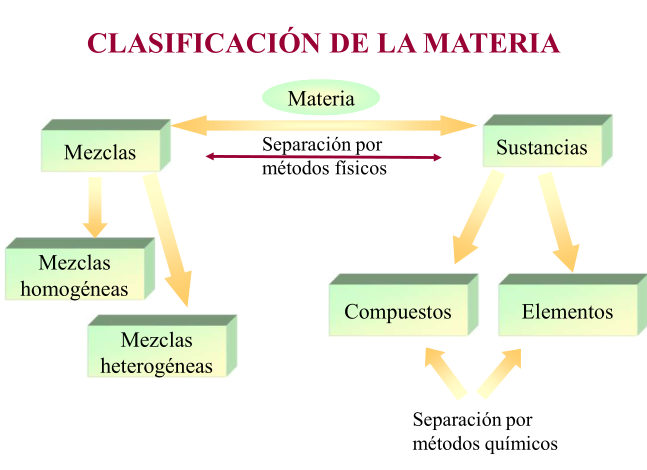
\includegraphics[width=6cm]{./imagenes/clasificacionMateria.png} \end{center}

        \indent La \textcolor{red}{\textit{Química}} es la ciencia que estudia la composición, estructura y propiedades de la materia, conjuntamente con los cambios que ésta sufre. \\
        \indent La \textcolor{red}{\textit{Materia}} es todo lo que ocupa lugar en el espacio y tiene masa. \\
        \indent Una \textcolor{red}{\textit{Sustancia}} es una forma de materia que tiene una composición dada y propiedades específicas que la distinguen de otras. \\
        \indent Una \textcolor{red}{\textit{Mezcla}} es una combinación de dos o más sustancias puras en la que cada una conserva sus propiedades particulares.

        \begin{itemize} 
            \item \textbf{Mezcla homogénea:} composición uniforme de la mezcla.
            \item \textbf{Mezcla heterogénea:} composición no uniforme de la mezcla.
        \end{itemize}   

        Los componentes de una mezcla se pueden separar mediante procesos físicos.

        \indent Un \textcolor{red}{\textit{Elemento}} es una sustancia que no se puede separar en otras más sencillas por medios químicos. \\
        \indent Un \textcolor{red}{compuesto} es una sustancia constituida por átomos de dos o más elementos químicos unidos en proporciones fijas definidas. \\
        Los compuestos sólo se pueden separar en sus elementos puros por medios químicos. \\
       
    \subsection{La materia (estados y propiedades)}
        \indent \textbf{\underline{Los estados de la materia son:}}
            \begin{itemize} 
                \item Sólido
                \item Líquido
                \item Gas
            \end{itemize}

        \indent \textbf{\underline{Cambios:}}
            \begin{itemize}
                \item \textcolor{red}{Físicos:} no altera la estructura o la identidad de una sustancia.
                \item \textcolor{red}{Químicos:} altera la estructura o identidad de la sustancias involucradas.
            \end{itemize}

        \indent \textbf{\underline{Propiedades:}}
            \begin{itemize}
                \item \textcolor{red}{Extensivas:} son aquellas dependientes de la cantidad de materia considerada.
                \item \textcolor{red}{Intensiva:} propiedad que no depende de la cantidad de materia considerada.
            \end{itemize}
            
        \indent \textbf{\underline{Átomos, moléculas e iones}}
            \begin{itemize}
                \item \textcolor{red}{Átomo:} partícula más pequeña de un elemento que mantiene su identidad química a través de todos los cambios físicos y químicos. Pueden intervenir en una combinación química. 
                \item \textcolor{red}{Molécula:} unión de dos o más átomos, eléctricamente neutros. Una molécula es la partícula más pequeña de un compuesto o elemento que tiene una existencia estable e independiente.
            \end{itemize}

            \begin{center} \underline{Representación del átomo} \end{center}
                \
        
